\subsection{Sprint 2}

Στην ενότητα αυτή παρουσιάζονται οι τιμές των μετρικών που
χρησιμοποιήθηκαν για κάθε κλάση/enumeration στο τέλος του sprint 2. Στο
τέλος του sprint 2 έχουν πια υλοποιηθεί αρκετές από τις κλάσεις γραφικής
διασύνδεσης της εφαρμογής. Πέρα από αυτές έχουν προστεθεί επίσης μερικές
βοηθητικές κλάσεις μικρού μεγέθους, με κώδικα που χρησιμοποιείται από
άλλες κλάσεις.

\subsubsection{Logical Lines Of Code (LLOC)}
\label{section:sprint2LLOC}

Στο σχήμα \ref{fig:sprint2LLOC} εμφανίζονται οι τιμές της μετρικής LLOC
για κάθε κλάση στο τέλος του sprint 2. Παρατηρούμε ότι οι κλάσεις με το
μεγαλύτερο μέγεθος είναι πια κυρίως οι κλάσεις γραφικής διασύνδεσης.
Αυτό είναι αναμενόμενο λόγω της φύσης του κώδικα που αφορά στη
διαχείριση γραφικών συστατικών. Αξίζει να σημειωθεί ότι ένα μεγάλο μέρος
του κώδικα στις κλάσεις γραφικής διασύνδεσης, αυτό που έχει να κάνει με
την τοποθέτηση των γραφικών συστατικών στα παράθυρα και τα σήματα που
εκτελούνται όταν ο χρήστης τα χρησιμοποιεί, έχει παραχθεί αυτόματα από
το λογισμικό JFormDesigner \cite{JFORMDESIGNER} που χρησιμοποιήθηκε για
το σχεδιασμό τους.

\begin{figure}
\centering
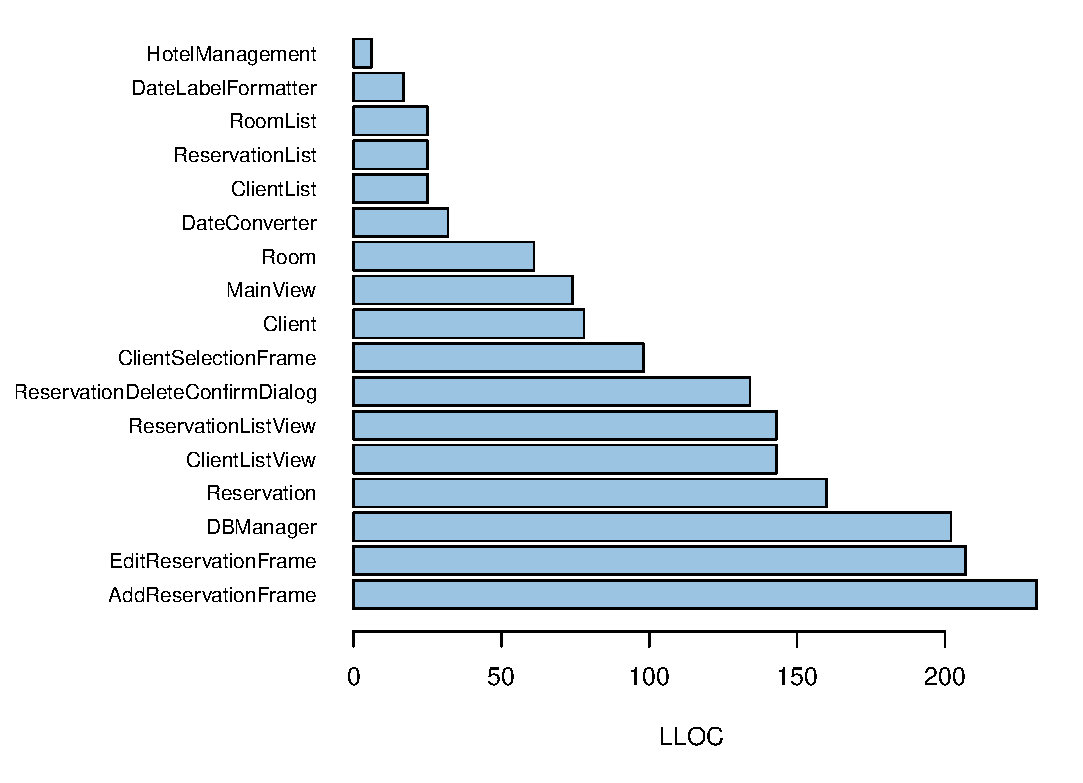
\includegraphics[width=1.0\textwidth]{Sprint2-LLOC-1.eps}
\caption{Λογικές γραμμές κώδικα ανά κλάση στο τέλος του sprint 2}
\label{fig:sprint2LLOC}
\end{figure}

Συγκεκριμένα, οι δύο κλάσεις με το μεγαλύτερο αριθμό λογικών γραμμών
κώδικα είναι οι AddRerservationFrame και EditReservationFrame, οι οποίες
υλοποιούν αντίστοιχα τα παράθυρα για την προσθήκη μιας κράτησης στο
σύστημα και την επεξεργασία μιας ήδη υπάρχουσας κράτησης. Και στις δύο
κλάσεις υπάρχει κώδικας για τον έλεγχο εγκυρότητας των στοιχείων που
δίνει ο χρήστης και τον έλεγχο διαθεσιμότητας σχετικά με την κράτηση. Οι
έλεγχοι αυτοί αποτελούν το μεγαλύτερο κομμάτι μη αυτόματα παραχθέντος
κώδικα που περιλαμβάνουν οι δύο κλάσεις. Δεδομένου ότι περίπου ο μισός
κώδικας των κλάσεων αυτών έχει παραχθεί αυτόματα και χειρίζεται τα
γραφικά συστατικά των αντίστοιχων παραθύρων, το μέγεθος των κλάσεων
κρίνεται ως μη ανησυχητικό.

Οι κλάσεις οντοτήτων που υλοποιούν τη backend λειτουργικότητα δεν έχουν
μεταβληθεί σε μέγεθος σε σχέση με αυτό που είχαν στο τέλος του sprint 1.

\subsubsection{Clone Coverage (CC)}
\label{section:sprint2CC}

Οι τιμές της μετρικής επανάληψης κώδικα CC για κάθε κλάση στο τέλος του
sprint 2 φαίνονται στο σχήμα \ref{fig:sprint2CC}. Παρατηρούμε ότι η
κλάση με τη μεγαλύτερη τιμή συνεχίζει να είναι η Client, ενώ και η κλάση
Room βρίσκεται στην τρίτη θέση χωρίς να έχει
αλλάξει η τιμή τους σε σχέση με το sprint 1. Η αιτιολόγηση των
φαινομενικά υψηλών τιμών τους είναι η ίδια με αυτή που διατυπώθηκε στην
ενότητα \ref{section:sprint1CC}.

\begin{figure}
\centering
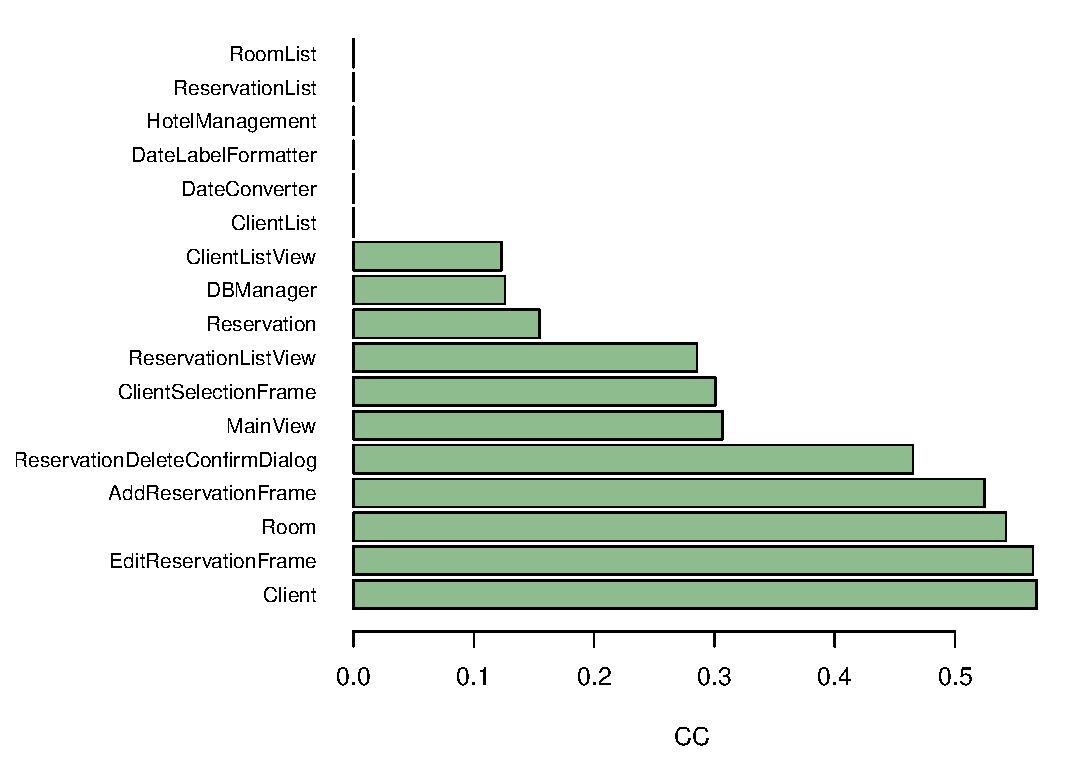
\includegraphics[width=1.0\textwidth]{Sprint2-CC-1.eps}
\caption{Τιμές της μετρικής CC ανά κλάση στο τέλος του sprint 2}
\label{fig:sprint2CC}
\end{figure}

Παρατηρούμε επίσης ότι υψηλές τιμές της μετρικής παρουσιάζουν και
κλάσεις γραφικής διασύνδεσης, με την κλάση EditReservationFrame να έχει
συνολικά τη δεύτερη μεγαλύτερη τιμή. Μετά από έλεγχο του κώδικα της
κλάσης, αλλά και των υπολοίπων κλάσεων γραφικής διασύνδεσης με επίσης
υψηλές τιμές, διαπιστώθηκε ότι η επαναληψιμότητα του κώδικα εμφανίζεται
στα κομμάτια του που έχουν παραχθεί αυτόματα. Είναι αναμενόμενο ότι ο
κώδικας διαχείρισης ενός γραφικού συστατικού, δηλαδή του κώδικα που
τοποθετεί, στέλνει και δέχεται σήματα, θα είναι όμοιος με τον
κώδικα που διαχειρίζεται ένα άλλο γραφικό συστατικό του ίδιου τύπου,
όπως για παράδειγμα μεταξύ του κώδικα που διαχειρίζεται δύο κουμπιά του
παραθύρου.

\subsubsection{McCabe's Cyclomatic Complexity (McCC)}
\label{section:sprint2McCC}

Στο σχήμα \ref{fig:sprint2McCC} εμφανίζονται οι τιμές της μετρικής
κυκλωματικής πολυπλοκότητας στο τέλος του sprint 2. Παρατηρούμε ότι η
κλάση Reservation είναι πια αυτή με την υψηλότερη τιμή. Πραγματικά, σε
αυτή προστέθηκαν αρκετές δομές ελέγχου σχετικές με τις κρατήσεις κατά τη
διάρκεια του sprint 2.

\begin{figure}
\centering
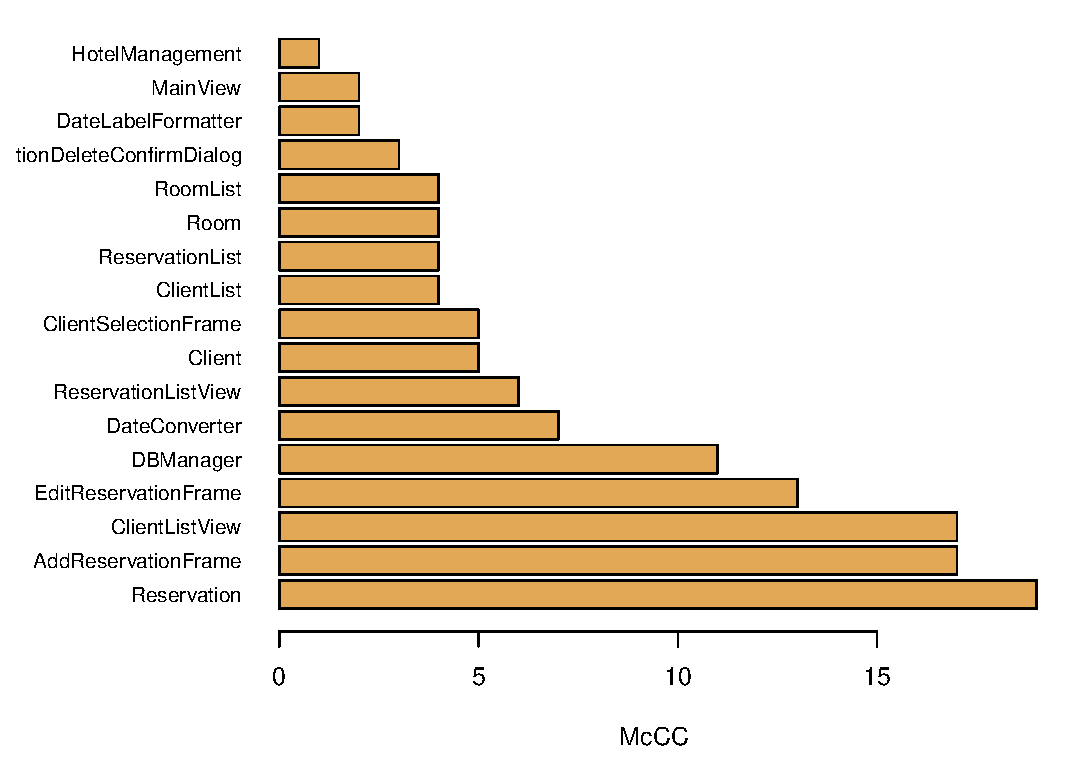
\includegraphics[width=1.0\textwidth]{Sprint2-McCC-1.eps}
\caption{Τιμές της μετρικής κυκλωματικής πολυπλοκότητας McCC ανά κλάση στο τέλος του sprint 2}
\label{fig:sprint2McCC}
\end{figure}

Άλλες κλάσεις με υψηλές τιμές είναι οι κλάσεις γραφικής διασύνδεσης που
σχετίζονται με τη δημιουργία και την επεξεργασία κρατήσεων. Κι αυτές
περιλαμβάνουν αρκετές δομές ελέγχου σχετικές με τον έλεγχο εγκυρότητας
και διαθεσιμότητας της κράτησης.

Πιθανόν να ήταν χρήσιμη η διάσπαση της κλάσης Reservation δύο
μικρότερες
για τη μείωση της τιμής της μετρικής McCC. Αντίστοιχα οι διάφοροι
έλεγχοι που οι κλάσεις γραφικής διασύνδεσης με υψηλές τιμές, θα
μπορούσαν πιθανόν να διαχωριστούν σε νέες κλάσεις, μειώνοντας τη
πολυπλοκότητά τους και ταυτόχρονα τη μέση τιμή της μετρικής για το
σύστημα. Το γεγονός όμως ότι όλες αυτές οι κλάσεις διατηρούν σχετικά
μικρό μέγεθος, κοντά στις 200 λογικές γραμμές κώδικα, σημαίνει ότι
μάλλον παραμένουν εύκολα διαχειρίσιμες ακόμα κι αν παραμείνουν ως έχουν.

\subsubsection{Lack of Cohesion in Methods 5 (LCOM5)}
\label{section:sprint2LCOM5}

Το σχήμα \ref{fig:sprint2LCOM5} παρουσιάζει τις τιμές της μετρικής
έλλειψης συνεκτικότητας LCOM5 για κάθε κλάση στο τέλος του sprint 2.
Παρατηρούμε και σε αυτή την περίπτωση ότι οι κλάσεις με τις υψηλότερες
τιμές είναι οι κλάσεις γραφικής διασύνδεσης που διαχειρίζονται τις
κρατήσεις.

\begin{figure}
\centering
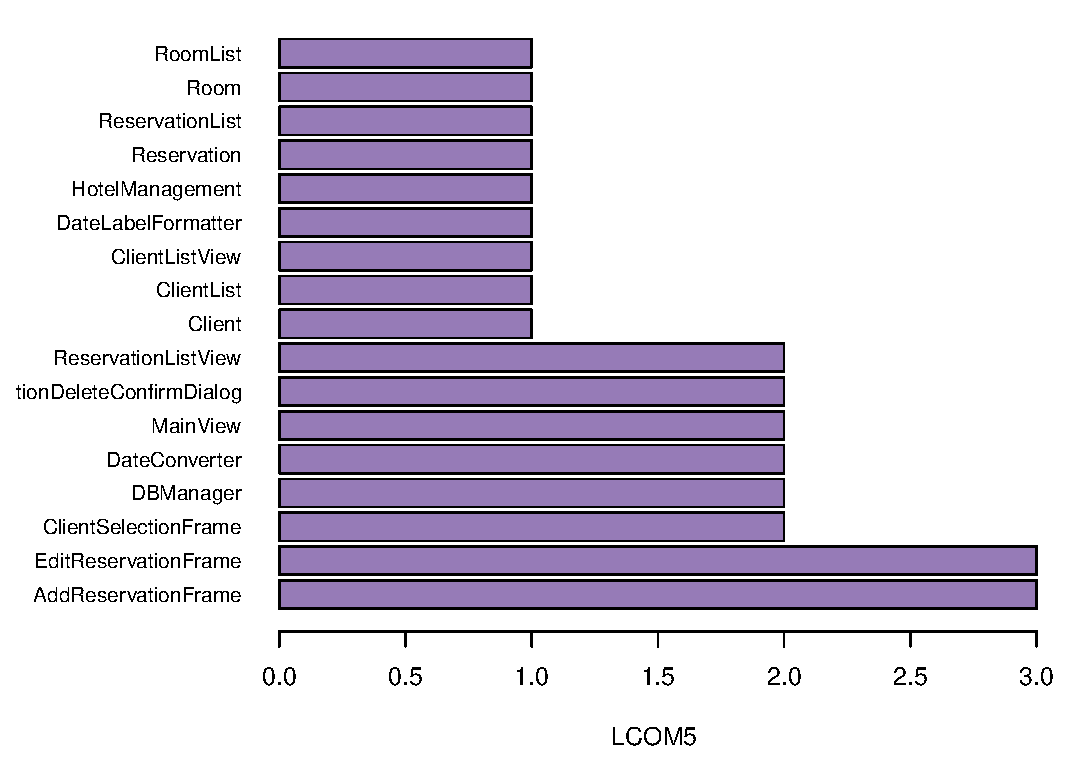
\includegraphics[width=1.0\textwidth]{Sprint2-LCOM5-1.eps}
\caption{Τιμές της μετρικής έλλειψης συνεκτικότητας LCOM5 ανά κλάση στο τέλος του sprint 2}
\label{fig:sprint2LCOM5}
\end{figure}

Αυτό αποτελεί ακόμα μία ένδειξη ότι οι κλάσεις αυτές θα
μπορούσαν να διασπαστούν σε μικρότερες σε μέγεθος κλάσεις, διαχωρίζοντας
τον κώδικα ελέγχου εγκυρότητας και διαθεσιμότητας των κρατήσεων σε
νέες κλάσεις.

\subsubsection{Coupling Between Object classes (CBO)}
\label{section:sprint2CBO}

Οι τιμές της μετρικής σύζευξης CBO για κάθε κλάση στο τέλος του sprint 2
εμφανίζονται στο σχήμα \ref{fig:sprint2CBO}. Παρατηρούμε ότι οι κλάσεις
γραφικής διασύνδεσης που σχετίζονται με τη διαχείριση κρατήσεων είναι
αυτές με τις υψηλότερες τιμές σύζευξης. Το γεγονός αυτό χαρακτηρίζεται
ως αναμενόμενο, αφού οι κρατήσεις περιλαμβάνουν στοιχεία πολλών άλλων
κλάσεων, όπως οι πελάτες, τα δωμάτια και τα αντίστοιχα παράθυρα δίνουν
στο χρήστη πληθώρα επιλογών για την προσθήκη, επεξεργασία και διαγραφή
κρατήσεων ή μεμονωμένων στοιχείων τους.

\begin{figure}
\centering
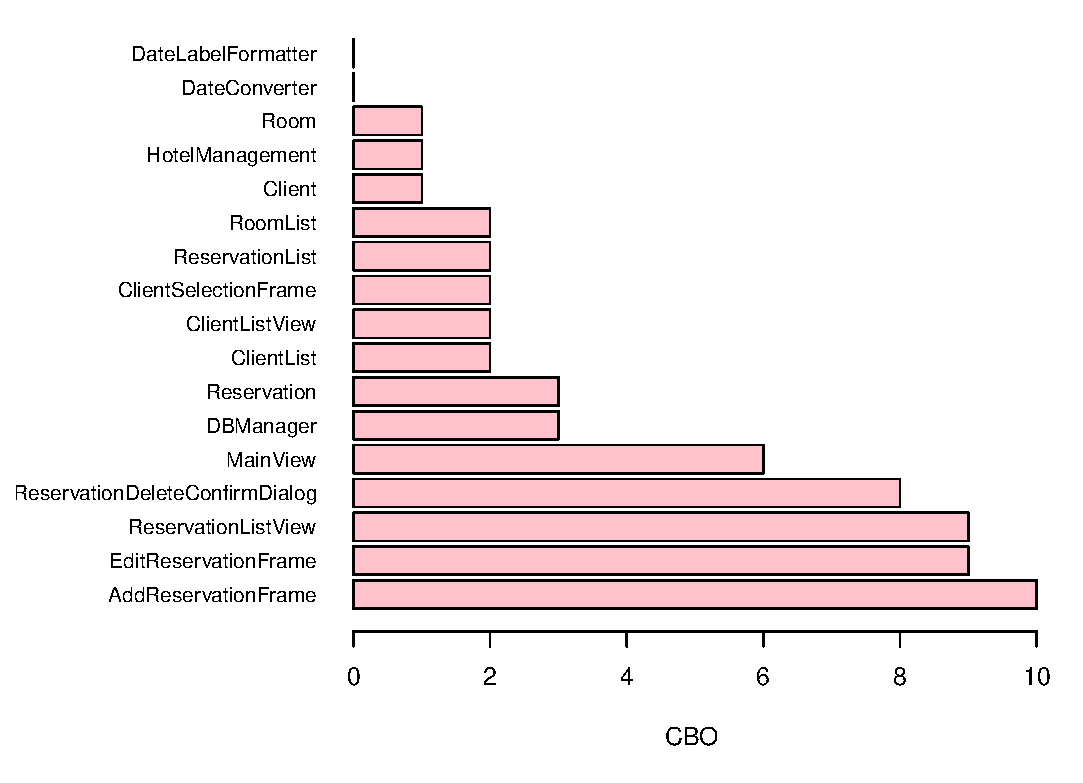
\includegraphics[width=1.0\textwidth]{Sprint2-CBO-1.eps}
\caption{Τιμές της μετρικής σύζευξης CBO ανά κλάση στο τέλος του sprint 2}
\label{fig:sprint2CBO}
\end{figure}
